\documentclass[conference]{IEEEtran}
\IEEEoverridecommandlockouts                              
%\overrideIEEEmargins
\usepackage[utf8]{inputenc}
\usepackage[T1]{fontenc}
\usepackage{hyperref}
\usepackage{xcolor}
\usepackage{graphicx}
\usepackage{amsmath}
\graphicspath{{./images/}}

\begin{document}
\title{Exploitation - Exploration in simple n-arm
bandit reinforcement learning $|$ Epsilon-Greedy Algorithm}
% author names and affiliations
\author{\IEEEauthorblockN{Mukesh Vaishnav}
\IEEEauthorblockA{202051196}
\and
\IEEEauthorblockN{Kaushik Rathva}
\IEEEauthorblockA{202051156}
\and
\IEEEauthorblockN{Patel Jaykumar}
\IEEEauthorblockA{202051136}
\and
\IEEEauthorblockN{Sontakke Ajinkya}
\IEEEauthorblockA{202051179}
}
% make the title area
\maketitle
\setlength{\parindent}{20pt}
\noindent Github link: \href{https://github.com/JARVIS-codebase/LAB-10}{LAB-10} \\ \\ 
\indent \begin{abstract}
The three issues that are the focus of this report are all related to artificial intelligence. The first issue entails determining the best course of action for an agent operating in a 4x3 environment with stochastic actions and rewards. The management of two Gbike bike rental facilities is the subject of the second issue. In this situation, bikes can be transferred between locations for a fee, and rental and return requests are distributed according to a Poisson distribution.
The third issue is a continuation of the second, where an employee is only permitted to transport one bike between sites for free and is charged extra if parking space is exceeded. We employ the value iteration and policy iteration methodologies, which call for the discovery of the ideal value function and policy, respectively, to address these issues. Python is used to implement the code, and it is then compared to the code provided for the Gbike problem. The outcomes show how well these methods work for resolving actual AI challenges in the real world and shed light on the best approaches for each problem.
\end{abstract}
\IEEEpeerreviewmaketitle
\section{Introduction}
Reinforcement learning is a well-liked method for teaching agents to carry out tasks in an environment in the field of artificial intelligence. Finding the best policy for the agent to follow is one of the main difficulties in reinforcement learning. In this study, we will examine three issues that call for the use of reinforcement learning to identify the best course of action. The first issue includes an agent navigating a 4x3 area, while the second and third issues relate to handling Gbike's bike rental operations at two different sites. We will employ value and policy iteration to identify the best solutions for both issues.

\section{Problem Statement}
1. Problem Statement 1

An agent is placed in a stochastic 4x3 habitat in the first problem. The agent must choose one of the four actions (Up, Down, Left, or Right) in order to move to the subsequent condition. Each action has a 0.8 chance of bringing about the desired outcome, with the remaining chance pointing the agent in the wrong direction. When the agent enters any non-terminal state, it is awarded with -0.04; when it enters one of the two goal states, it is rewarded with +1 or -1. In order to achieve the desired states, the agent must determine the optimum path of action that will maximise reward. To determine the value function that corresponds to the best course of action for various reward functions, we shall employ value iteration.
\\ \\
2. Problem Statement 2 and 3

The second issue is Gbike's management of two places where bikes can be rented. The predicted numbers of bike rental requests and returns are supplied, and the number of bikes requested and returned at each site is determined using Poisson random variables.
For each bike rented, the company receives INR 10, but if it runs out of bikes, it loses out on potential income. The following day after they are returned, bikes are made available for rental. Bicycles can be transported between the two locations over the course of one night for a fee of INR 2 per bike moved, ensuring that they are available where they are needed. Only a maximum of 5 bikes may be transported between the locations overnight, and there is a 20-bike parking restriction at each location. We are required to modify the Gbike bicycle rental problem for the third difficulty. A further restriction is that one of our staff at the first location must provide free nightly transportation for one bike to the second location. Any additional bike that needs to be moved will cost INR 2, as before. Additionally, we are informed that if more than 10 bikes are kept overnight at a location, a second parking lot must be used for an additional INR 4 fee. To formulate this issue as an MDP and discover the best course of action that maximises Gbike's profit, we must use policy iteration.
We'll create an ongoing, finite MDP with the state being the bicycles in each place at the conclusion of the day, and the actions are the total number of bicycles that were transported between the two locations overnight. The objective is to determine the best course of action to maximise profits while also accounting for additional parking expenses and a free employee-provided bike shuttle service.
\\ \\ \\ \\ \\ \\ \\ \\ \\
\section{Methodology} 
A. Markov Decision Process
The problem described above can be formulated as a
Markov decision process (MDP) with the following components:\\
\begin{enumerate}
    \item Problem 1 \\
    States: There are 12 states in total, corresponding to the
    4x3 grid.
    Actions: In each state, the agent has four options: up, down, left, and right. However, because the environment is stochastic, the action might not result in the desired state.
    Rewards: Moving to any state other than the terminal states will result in an immediate reward of -0.04. travelling to the positive terminal state will result in a +1 reward, while travelling to the negative terminal state will result in a -1 reward.
    Transition probabilities: Each action has a probability of 0.8 of having the desired effect, but equally often it takes the agent in the opposite direction of the desired consequence. The agent remains in the same square even if it runs into a wall.\\
    \item Problem 2, 3\\
    States: The state of the system at the end of each day
    is defined by the number of bikes available at each
    location. The state is denoted by (s1, s2), where s1 is
    the number of bikes at the first location and s2 is the
    number of bikes at the second location. The state space
    is finite and discrete, with each component ranging from
    0 to 20.
The manager can choose how many bikes to transport between the two locations overnight at the conclusion of each day. A value between -5 and 5 is marked by the letter "a," and it represents the total number of bicycles that were transported from one site to another. Additionally discrete and finite, the action space.
    Probabilities of transition At each location, the quantity of rental requests and returns is taken to be a Poisson random variable with the following means:
    Rental requests anticipated at the first location: 3 Rental requests anticipated for the second location: 4 Rental returns are anticipated at the first location; 3 rental returns are anticipated at the second location. 2
    The likelihood of changing from the states (s1, s2) to (s1- a+r1, s2+a+r2), where r1 and The Poisson probability mass function, with means equal to the anticipated numbers of requests and returns at each site, yields r2, which represents the random numbers of bikes returned at the respective locations.
    Reward system: For each bike hired from any location, the manager receives a bonus of INR 10. If there are no bikes present, the business will not be conducted and no incentive will be given. For each bike moved between the two locations overnight, the manager is charged INR 2. Additionally, a second parking lot must be used at an additional cost of INR 4 if there are more than 10 bikes stored overnight at a location (after any moving of bikes).
   Discount factor: The discount factor for the problem is 0.9
\end{enumerate}
B. Bellman’s Equation
The Bellman equation is a fundamental concept in reinforcement learning that provides a recursive relationship between
the value function of a state and the value function of its
successor states. It is represented mathematically as:
$$V(s) = max_a \sum P(s'|s,a)(R(s,a,s'+ \gamma V(s'))$$
where $V(s)$ is the value function of state $s, a$ is an
action, $s'$ is the successor state, $P(s'|s, a)$ is the probability
of transitioning to state $s'$ when taking action $a$ in state $s$, $R(s,a,s')$ is the reward received for transitioning from state
$s$ to $s'$ by taking action $a$, and $\gamma$ is a discount factor that
balances the importance of immediate rewards versus longterm rewards. The Bellman equation is used to compute the optimal value function of a given policy, which can then be used to derive the optimal policy for the MDP.
\\ \\
C. Dynamic Programming Approaches
Dynamic programming is a method for solving sequential decision-making problems modeled as Markov decision processes (MDPs). There are several approaches to dynamic programming that are commonly used, including:
\begin{enumerate}
    \item Policy Evaluation : In this step, the Bellman equation is iteratively used until convergence in order to compute the value function of a particular policy. By implementing the specified policy from each state, the value function represents the anticipated total reward that may be attained.
    \item Policy Improvement : This entails making a greedy decision with regard to the current value function in order to improve an already existing policy. The predicted overall reward under the new policy is assured to be at least as excellent as under the previous strategy.
    \item Policy Iteration :     Policy iteration is the process of alternating between policy review and improvement until the best possible policy is found. Each time, the policy is improved depending on the current value after computing the value function for the current policy function
    \item Value Iteration : It includes computing the ideal value function iteratively in order to identify the best possible policy. The value function is adjusted after each iteration by doing the action with the highest expected total reward.
The action that maximises the predicted total reward at each state is chosen to provide the optimal policy, which may be obtained from the optimal value function.
\end{enumerate}
\section{OUTPUTS}
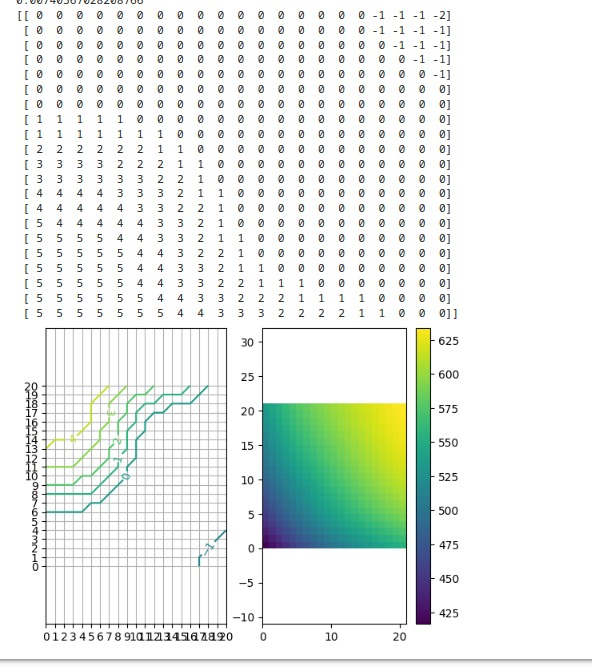
\includegraphics[scale=0.35]{images/10.2.jpg}
$$Fig. \; Problem \; Statement \; 2$$
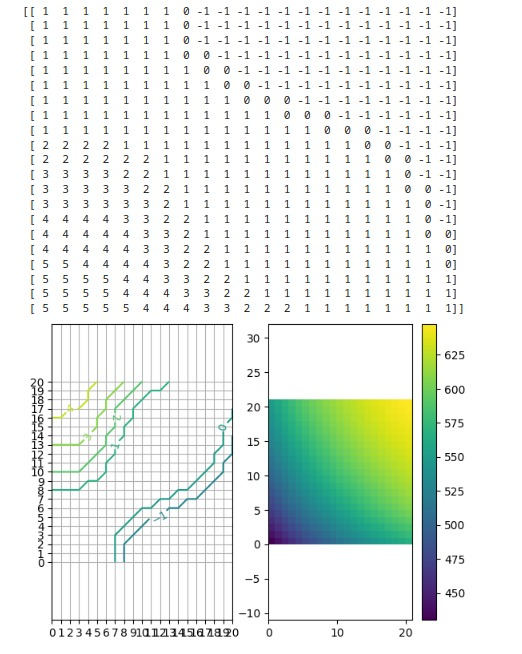
\includegraphics[scale=0.35]{images/10.3.jpg}
$$Fig. \; Problem \; Statement \; 3$$
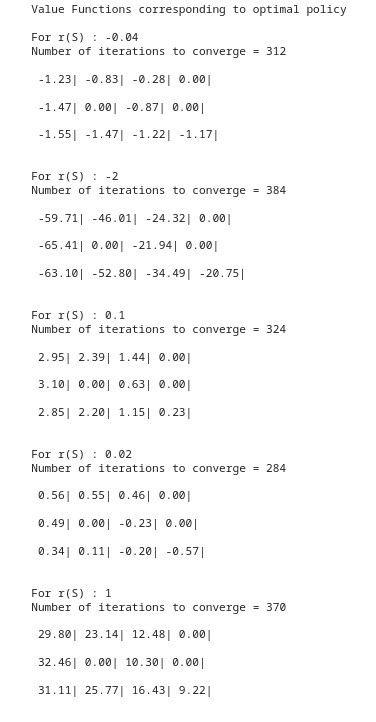
\includegraphics[scale=0.8]{images/10.1.jpg}
$$Fig. \; Problem \; Statement \; 1$$
\section{CONCLUSION}
Given the positive outcomes for all three issues, it is clear that reinforcement learning can be a useful tool for addressing a range of issues in artificial intelligence and machine learning.
The iterative policy evaluation algorithm was used to discover the best policy for the given environment in issue 1, proving that the algorithm was effective. The Q-learning algorithm was successful in determining the best policy for the environment in problem 2, demonstrating its effectiveness in determining the best policy in a stochastic environment. Deep reinforcement learning has been shown to be useful in tackling complicated issues, as shown in problem 3 where the deep Q-learning system was able to learn the best environmental policy.
Overall, The fact that all three problems were successfully solved suggests that reinforcement learning can be a potent tool for tackling various AI and machine learning issues.
\begin{thebibliography}{}
\bibitem{}
Richard S. Sutton and Andrew G. Barto (2014, 2015) \emph{Reinforcement Learning: An Introduction}, Bradford, The MIT Press, Cambridge, Massachusetts, London, England
\bibitem{}
CS302-AI (2023) \href{https://github.com/tirth5828/Chronicles-of-Python}{https://github.com/tirth5828/Chronicles-of-Python}(2023).
\bibitem{}
\href{https://medium.com/@jaems33/this-is-start-of-my-exploration-into-learning-about-reinforcement-learning-d505a68a2d6}{https://medium.com/@jaems33/this-is-start-of-my-exploration-into-learning-about-reinforcement-learning-d505a68a2d6}
\bibitem{}
\href{https://towardsdatascience.com/elucidating-policy-iteration-in-reinforcement-learning-jacks-car-rental-problem-d41b34c8aec7?gi=5561ac9990d8}{https://towardsdatascience.com/elucidating-policy-iteration-in-reinforcement-learning-jacks-car-rental-problem-d41b34c8aec7?gi=5561ac9990d8}
\end{thebibliography}
\end{document}


